\documentclass[11pt,openright,a4paper]{report}
\usepackage{graphicx}
\usepackage{pdflscape}
\usepackage{hyperref}
\graphicspath{ {images/} }

\title{Using Machine-learning Techniques to Increase the Effiency of Kinect Fusion Reconstructions}
\author{Alan Lau Wing Leung}
\date{MComp Computer Science\\University of Bath\\October 2015}

% reduce Chapter margin size
\makeatletter
\def\@makechapterhead#1{%
  %%%%\vspace*{50\p@}% %%% removed!
  {\parindent \z@ \raggedright \normalfont
    \ifnum \c@secnumdepth >\m@ne
        \huge\bfseries \@chapapp\space \thechapter
        \par\nobreak
        \vskip 20\p@
    \fi
    \interlinepenalty\@M
    \Huge \bfseries #1\par\nobreak
    \vskip 40\p@
  }}
\def\@makeschapterhead#1{%
  %%%%%\vspace*{50\p@}% %%% removed!
  {\parindent \z@ \raggedright
    \normalfont
    \interlinepenalty\@M
    \Huge \bfseries  #1\par\nobreak
    \vskip 40\p@
  }}
\makeatother





\begin{document}

\maketitle
\newpage

\tableofcontents
\newpage

% reset page number
\setcounter{page}{1}

% problem description
\chapter{Problem Description}
Kinect Fusion is a Micrsoft Research project that enables rapid and detailed 3D reconstructions, both real-time and off-line, through scanning an object and merging the depth data of many frames together, with the help of a Kinect camera [1][2].

A few research projects from Microsoft demonstrate some interesting ideas about the possibilities of Kinect Fusion. For example, SemanticPaint [3] provides a real-time augmented experience where users can label and segment through the combination of commands, Kinect Fusion and object recognition, allowing different objects to be painted in the reconstruction in real-time. Other researches include non-rigid scene reconstruction [4], dense surface mapping [5] and a Master's thesis on building-scale interior reconstruction. [6] These and other similar projects will be become useful information when attempting this project.

One issue with Kinect Fusion is that it does not store and recognise objects it has seen before. This means that a seen object will require the same reconstruction again, making it inefficient when trying to obtain reconstructions in scenes with the same or similar objects.

This project aims to solve this with the help of a classifier. For instance, many rooms at the University share the same equipment across multiple rooms. Rather than having to re-scan and reconstruct an object encountered before, a newly reconstructed item should be stored and be identified by the classifier later. When encountering a new scene with the same object in it, only a quick scan from one angle is needed to fill in the full, detailed scans of objects seen before. This shortens the time and minimise the effort required to reconstruct a new scene with identical objects, but provides a fairly accurate and detailed reconstruction at the same time.

As a classifier is used, it should should be able to locate the best match anyway. The best matched item could be put in place with a one-angled quick scan for a new scene with new but similar objects in it (e.g. a similar round table). If it is deemed good enough, the room reconstruction can be used, without the need of further scanning. If further scanning of an object is required, it can then replace an object of the reconstructed scene at a later time.

\section{Aim}
The aim is to quickly reconstruct a scene without needing to re-scan each object in detail again to obtain a well-reconstructed scene, by using classifiers or other appropriate machine-learning techniques.

\section{Objectives}
\subsection{Main Objectives}
\begin{enumerate}
  \item Develop one or a set of classifiers that can accurately identify a seen object or able to find the next best match if it does not exist.
  \item Vigorously train and test the classifier with many scans of similar objects to improve its accuracy
  \item Design and implement algorithms to locate potential object positions and obtain the partial information
  \item Integrate the classifier with the algorithms to create a reconstructed scene using the identified reconstructions
\end{enumerate}

\subsection{Stretched Objectives}
These objectives are nice to have if they can be done on top of the main objectives, but it is expected these will not be achievable with the limited time and scope of this project.
\begin{enumerate}
  \item Adapt and develop a real-time version where objects are being put in place right at the scene
  \item Provide an augmented reality experience similar to SemanticPaint [3] - one that allows real-time recognition and colouring.
\end{enumerate}

\newpage

% Requirements Specification
\chapter{Requirements Specification}

\begin{enumerate}
  \item The classifier needs to be accurate in recognising and discerning between different objects.
    \begin{itemize}
      \item Precision and Recall needs to be high enough to be useful.
      \item NYU Depth Dataset [7] can be used to in early prototype classifiers.
      \item The classifier, especially the prototypes, must use a simple language (e.g. \textit{R}, \textit{Python}) for quick iteration.
    \end{itemize}
  \item Training of the classifier requires a large dataset to make it accurate.
    \begin{itemize}
      \item Utilise the NYU Depth Dataset [7] as the basis of training the classifier, alongside with scans made of objects at the University.
    \end{itemize}
  \item The algorithms for locating and filling in objects need to be fairly accurate.
    \begin{itemize}
      \item Otherwise, the objects not be fitted at the right place and makes the reconstruction inaccurate.
    \end{itemize} 
\end{enumerate}

\newpage


% Project Plan
\chapter{Project Plan}
\section{Project Management}
There are three main elements in this project:
\begin{enumerate}
  \item a classifier that finds out the object in disguise;
  \item an algorithms that figures out where the missing bits are; and,
  \item combinding the two to obtain a reconstructed scene.
\end{enumerate}

In order to complete these complicated implementations, much organisation and reading up are needed. I plan to iterate 4 times (2 weeks or so at a time) on the coding side of things for both the classifier and algorithms, starting on 1 November. This is to ensure that timely and achievable goals are set and that problems can be resolved as soon as it is discovered.

I intend not to work on the project during the three-week examination period, as realistically, most effort will be put in revision and there will be little time for other work.

A five-week period during February and March will be used to finalise the codebase. Five weeks are set apart for writing up the dissertation. This should provide enough time to handle any delay, development complications and for the disseration write-up. 

\textit{See [Appendix A] for the gant chart.}

\newpage


% Resources
\chapter{Resources}

\section{Technologies}
\begin{enumerate}
  \item A simple language and fast library is required for easy iteration. 
  \begin{itemize}
    \item \textit{R} or \textit{Python} (with the libraries such as \textit{pyML}, \textit{numpy} or \textit{scikit-learn}) can be used to produce the classifier. They are languages that are easy to code with and are used for handling data.
    \item Initially, the large library of Kinect data from NYU (The NYU Depth Dataset) [7] should be used while constructing the classifier. This provides a good selection of data and understanding how to interpret them.
  \end{itemize}
  
  \item Kinect Fusion and the Kinect for Windows SDK
  \begin{itemize}
    \item These SDKs are needed to for capturing depth data. They need to be installed on a PC running Windows.
    \item Other related packages such as Visual Studio may be required to allow capturing and other manipulation.
  \end{itemize}
\end{enumerate}

\section{Hardware}
  \begin{enumerate}
    \item A relatively powerful Windows-based computer with a (preferably, discrete) graphics card that supports DirectX 11.
      \begin{itemize}
        A DirectX 11-supported graphics card required for Kinect Fusion to function properly. 
      \end{itemize}
    \item Kinect for Windows
      \begin{itemize}
        \item For capturing the depth data.
      \end{itemize}
  \end{enumerate}

\newpage


% Appendix
\begin{landscape}
\chapter{Appendix}
\section{Appendix A}
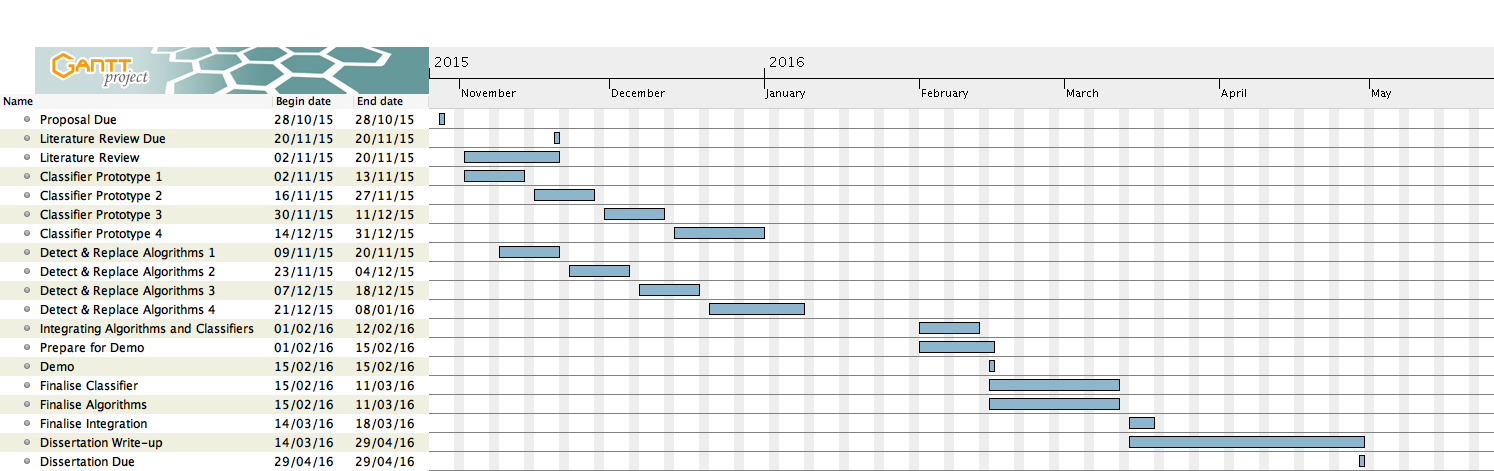
\includegraphics[scale=0.38,keepaspectratio]{gant}
\end{landscape}
\newpage


% References
\begin{thebibliography}{7}
  \bibitem{msdn-kinect-info}
    Microsoft Corporation.
    \textit{Kinect Fusion} [Online]. 
    Place of publication: Microsoft Developer Network.
    Available from: \url{https://msdn.microsoft.com/en-us/library/dn188670.aspx}
    [Accessed 22 October 2015].

  \bibitem{blog-kinect-annc}
    Kinect for Windows Team, 2013.
    \textit{Kinect Fusion demonstrated at Microsoft Research TechFest, coming soon to SDK} [Online].
    Place of publication: Kinect for Windows Blog
    Available from: \url{http://blogs.msdn.com/b/kinectforwindows/archive/2013/03/06/kinect-fusion-demonstrated-at-microsoft-research-techfest-coming-soon-to-sdk.aspx}
    [Accessed 22 October 2015].

  \bibitem{blog-semantic-paint}
    Cameron, S., 2015.
    \textit{Microsoft Research debuts another project, Semantic Paint} [Online].
    Place of publication: WinBeta Blog
    Available from: \url{http://www.winbeta.org/news/microsoft-research-debuts-another-project-semantic-paint}
    [Accessed 23 October 2015].

  \bibitem{art-DyanmicFusion}
    Newcombe, R. A. et al., 2015.
    DynamicFusion: Reconstruction and Tracking of Non-rigid Scenes in Real-Time. 
    \textit{Proceedings of the IEEE Conference on Computer Vision and Pattern Recognition}, 7-12 June 2015 Boston, Massachusetts.
    Seatle: University of Washington, pp.343-352.
    %Available from: \url{http://homes.cs.washington.edu/~newcombe/papers/DynamicFusion.pdf}
    %[Accessed 23 October 2015].

  \bibitem{art-dense-surface}
    Newcombe, R A et al., 2011.
    KinectFusion: Real-time dense surface mapping and tracking.
    \textit{Mixed and augmented reality (ISMAR), 2011 10th IEEE international symposium}, 26-29 October 2011 Basel, Switzerland.
    Seatle: University of Washington, pp.127-136
    %Available from: \url{http://homes.cs.washington.edu/~newcombe/papers/newcombe_etal_ismar2011.pdf}
    %[Accessed 23 October 2015].

  \bibitem{the-HouseScan}
    Hambüchen, N., 2014.
    \textit{HouseScan: Building-scale interior 3D reconstruction with KinectFusion}. 
    Thesis (MSc).
    Imperial College, London.
    %Available from: \url{http://www.doc.ic.ac.uk/teaching/distinguished-projects/2014/n.hambuechen.pdf}
    %[Accessed 23 October 2015].

  \bibitem{}
    Silberman, N. et al..
    \textit{NYU Depth Dataset V2} [Online].
    Available from: \url{http://cs.nyu.edu/~silberman/datasets/nyu_depth_v2.html}
    [Accessed 23 October 2015].

\end{thebibliography}
\newpage


\end{document}
